% !TEX root = ./thesis.tex

\chapter*{\textbf{Appendix 2: Workshop Materials \\ \hspace{1em}}}
\addcontentsline{toc}{chapter}{Appendix 2: Chapter II Workshop Materials}

\setcounter{chapter}{4}
\setcounter{table}{0}
\setcounter{figure}{0}

This appendix contains documents relevant to the stakeholder workshop of Chapter 2: 
\begin{itemize}
  \item \textbf{Feuille de route du Participant - Workshop participant roadmap} - This is the document that was given to each participant during the workshop. It contains helpful information meant to guide them during the exercises: the agenda for the day, a few illustrations of simple connectivity concepts, and suggestions of assets and obstacles to connectivity.
  % \item \textbf{Document du facilitateur - Facilitator's sheet} - This is the document that was given to each facilitator. It contains guidelines for leading the conversation at each table and at each step of the workshop.
  % This needs to be removed for final submission.
  % \item \textbf{Certificate of Ethical Acceptability of Research Involving Humans} - This document certifies that this research project was approved by McGill's university Research Ethics Board Office.
\end{itemize}

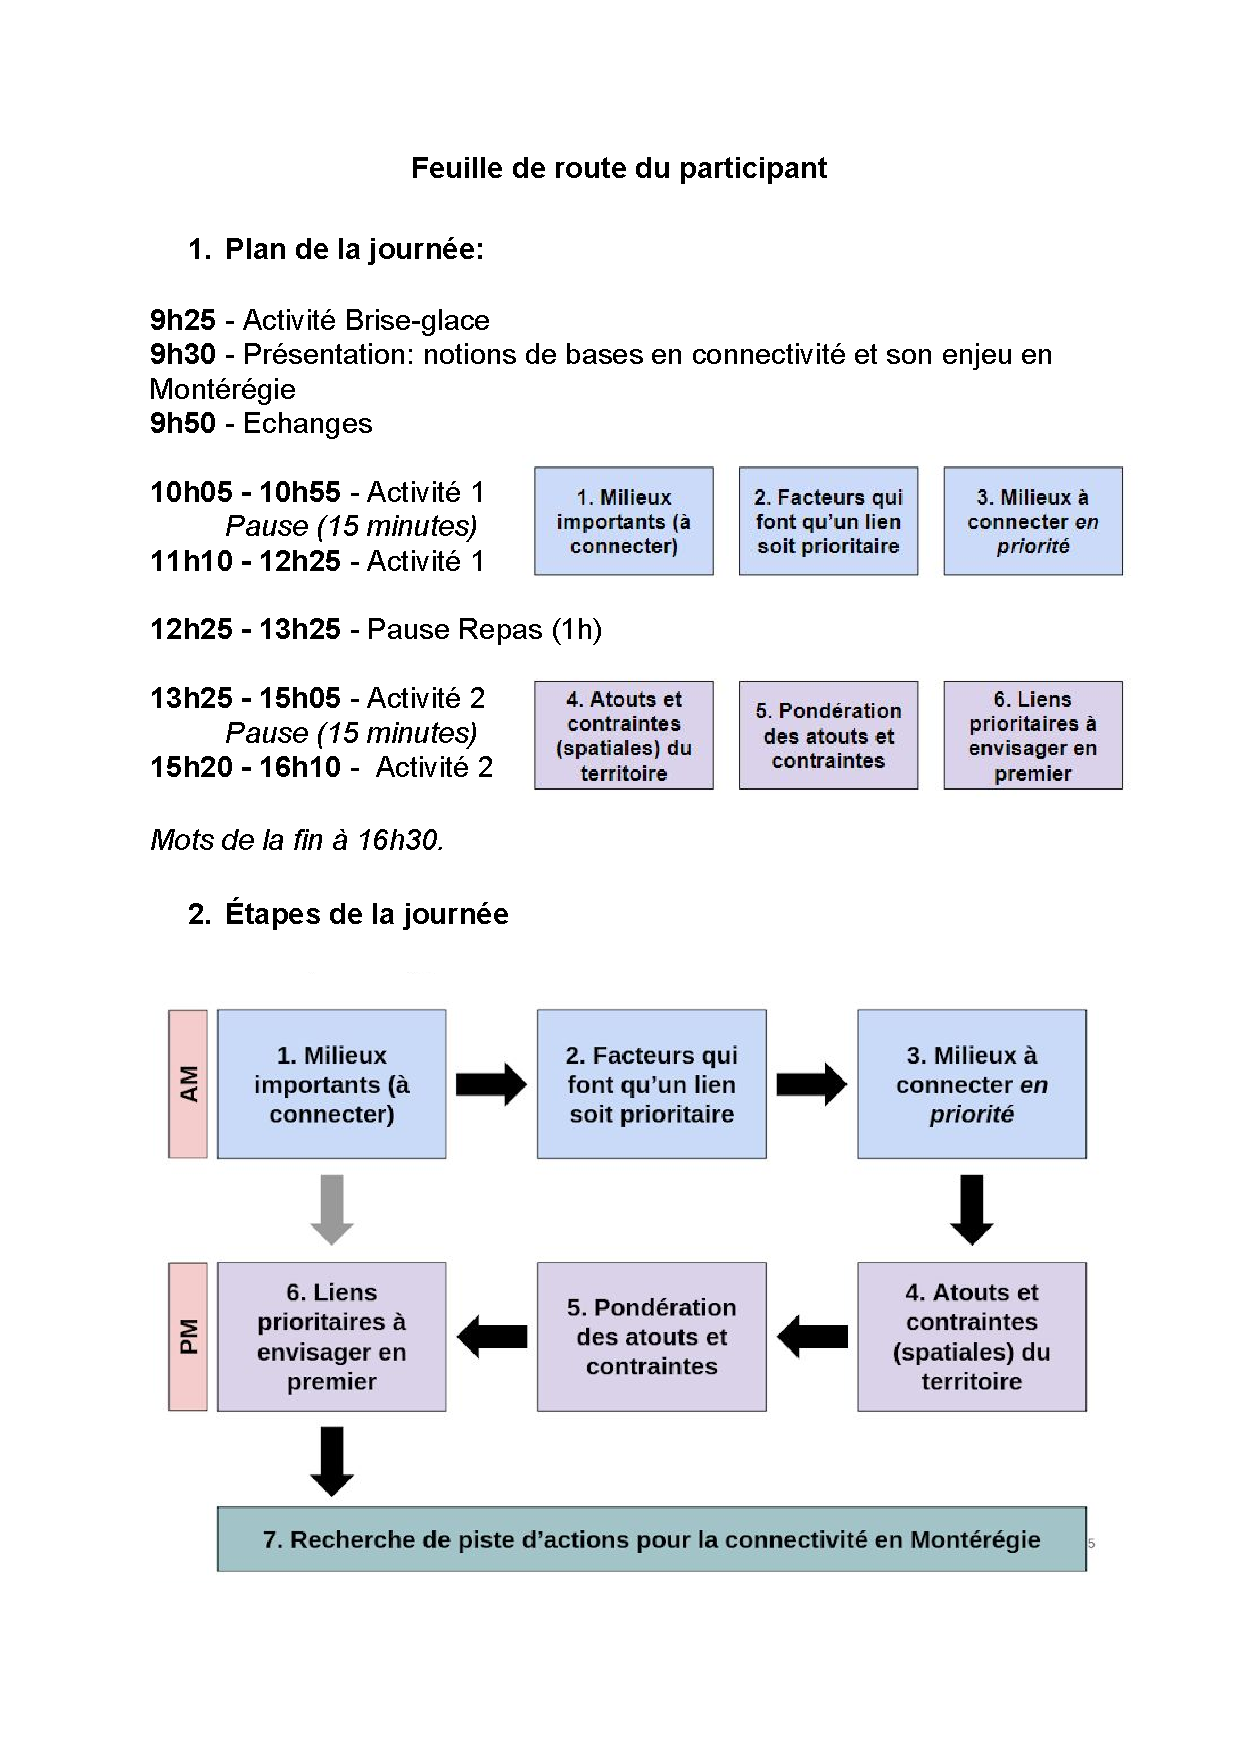
\includepdf[pages=-,pagecommand={},width=1.3\textwidth]{thesis/appendix/Cahier_du_Participant.pdf}
% \includepdf[pages=-,pagecommand={},width=1.3\textwidth]{thesis/appendix/Document_du_facilitateur.pdf}
% 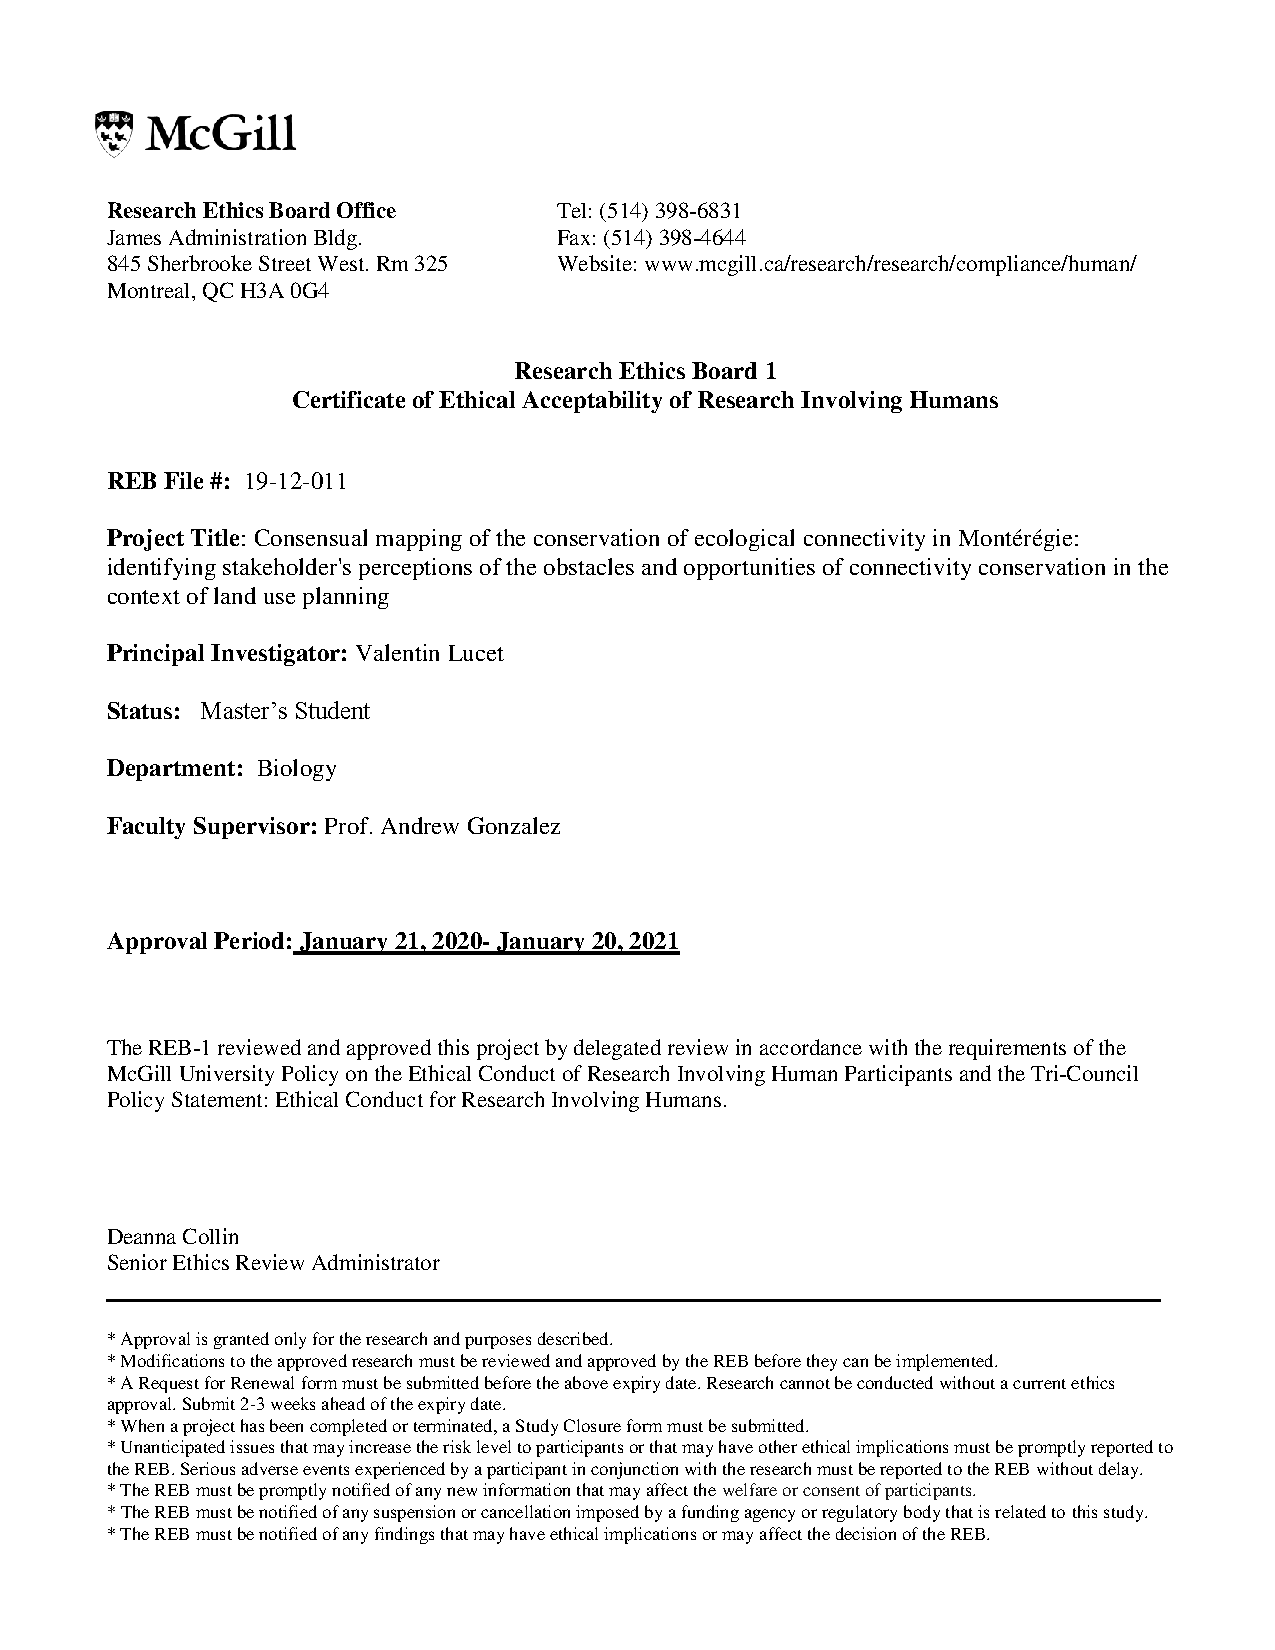
\includepdf[pages=-,pagecommand={},width=1.3\textwidth]{thesis/appendix/Ethics_approval_Lucet.pdf}